\chapter{\texorpdfstring{Process Mining}{Process Mining}}
\label{ch:05}
\lecturemeta{Lezione 05 \quad\textbullet\quad 2026-07-03 \quad\textbullet\quad Roberto Bruni}{van der Aalst, \emph{Process Mining}, Ch.1 e 6}

Fino a qui abbiamo imparato a \emph{disegnare} un processo e a dargli una semantica formale con i \hyperref[ch:04]{Petri net}. Ma da dove viene il modello? Finora l'abbiamo sempre supposto dato, disegnato a mano da un analista. Il \textbf{process mining} ribalta la prospettiva: invece di \emph{progettare} il modello e poi confrontarlo con la realtà, parte dai \textbf{dati reali} — le tracce che i sistemi informatici lasciano mentre eseguono i processi — e da lì \emph{scopre}, monitora e migliora il processo effettivo.

\begin{boxdefinition}{Process mining}
Una disciplina di ricerca relativamente giovane che si colloca \textbf{tra} il \emph{machine learning / data mining} da un lato e il \emph{process modeling / analysis} dall'altro. L'idea è \textbf{scoprire, monitorare e migliorare} i processi reali estraendo conoscenza dagli \textbf{event log} già disponibili nei sistemi odierni.
\end{boxdefinition}

Il punto di forza è che non lavora su ciò che le persone \emph{dicono} di fare, ma su ciò che il sistema \emph{registra} essere stato fatto. È la differenza tra intervistare gli impiegati e leggere i log del gestionale.

\section{\texorpdfstring{Lo schema del process mining}{Lo schema del process mining}}

Tutta la disciplina si organizza attorno a uno schema che mette in relazione tre elementi: il \textbf{"world"} (il mondo reale con persone, macchine, organizzazioni e i loro business process), il \textbf{software system} che supporta e controlla quel mondo, e i \textbf{process model} che ne descrivono la logica. Tra questi elementi scorrono informazioni in entrambe le direzioni.

\begin{figure}[!htb]
\centering
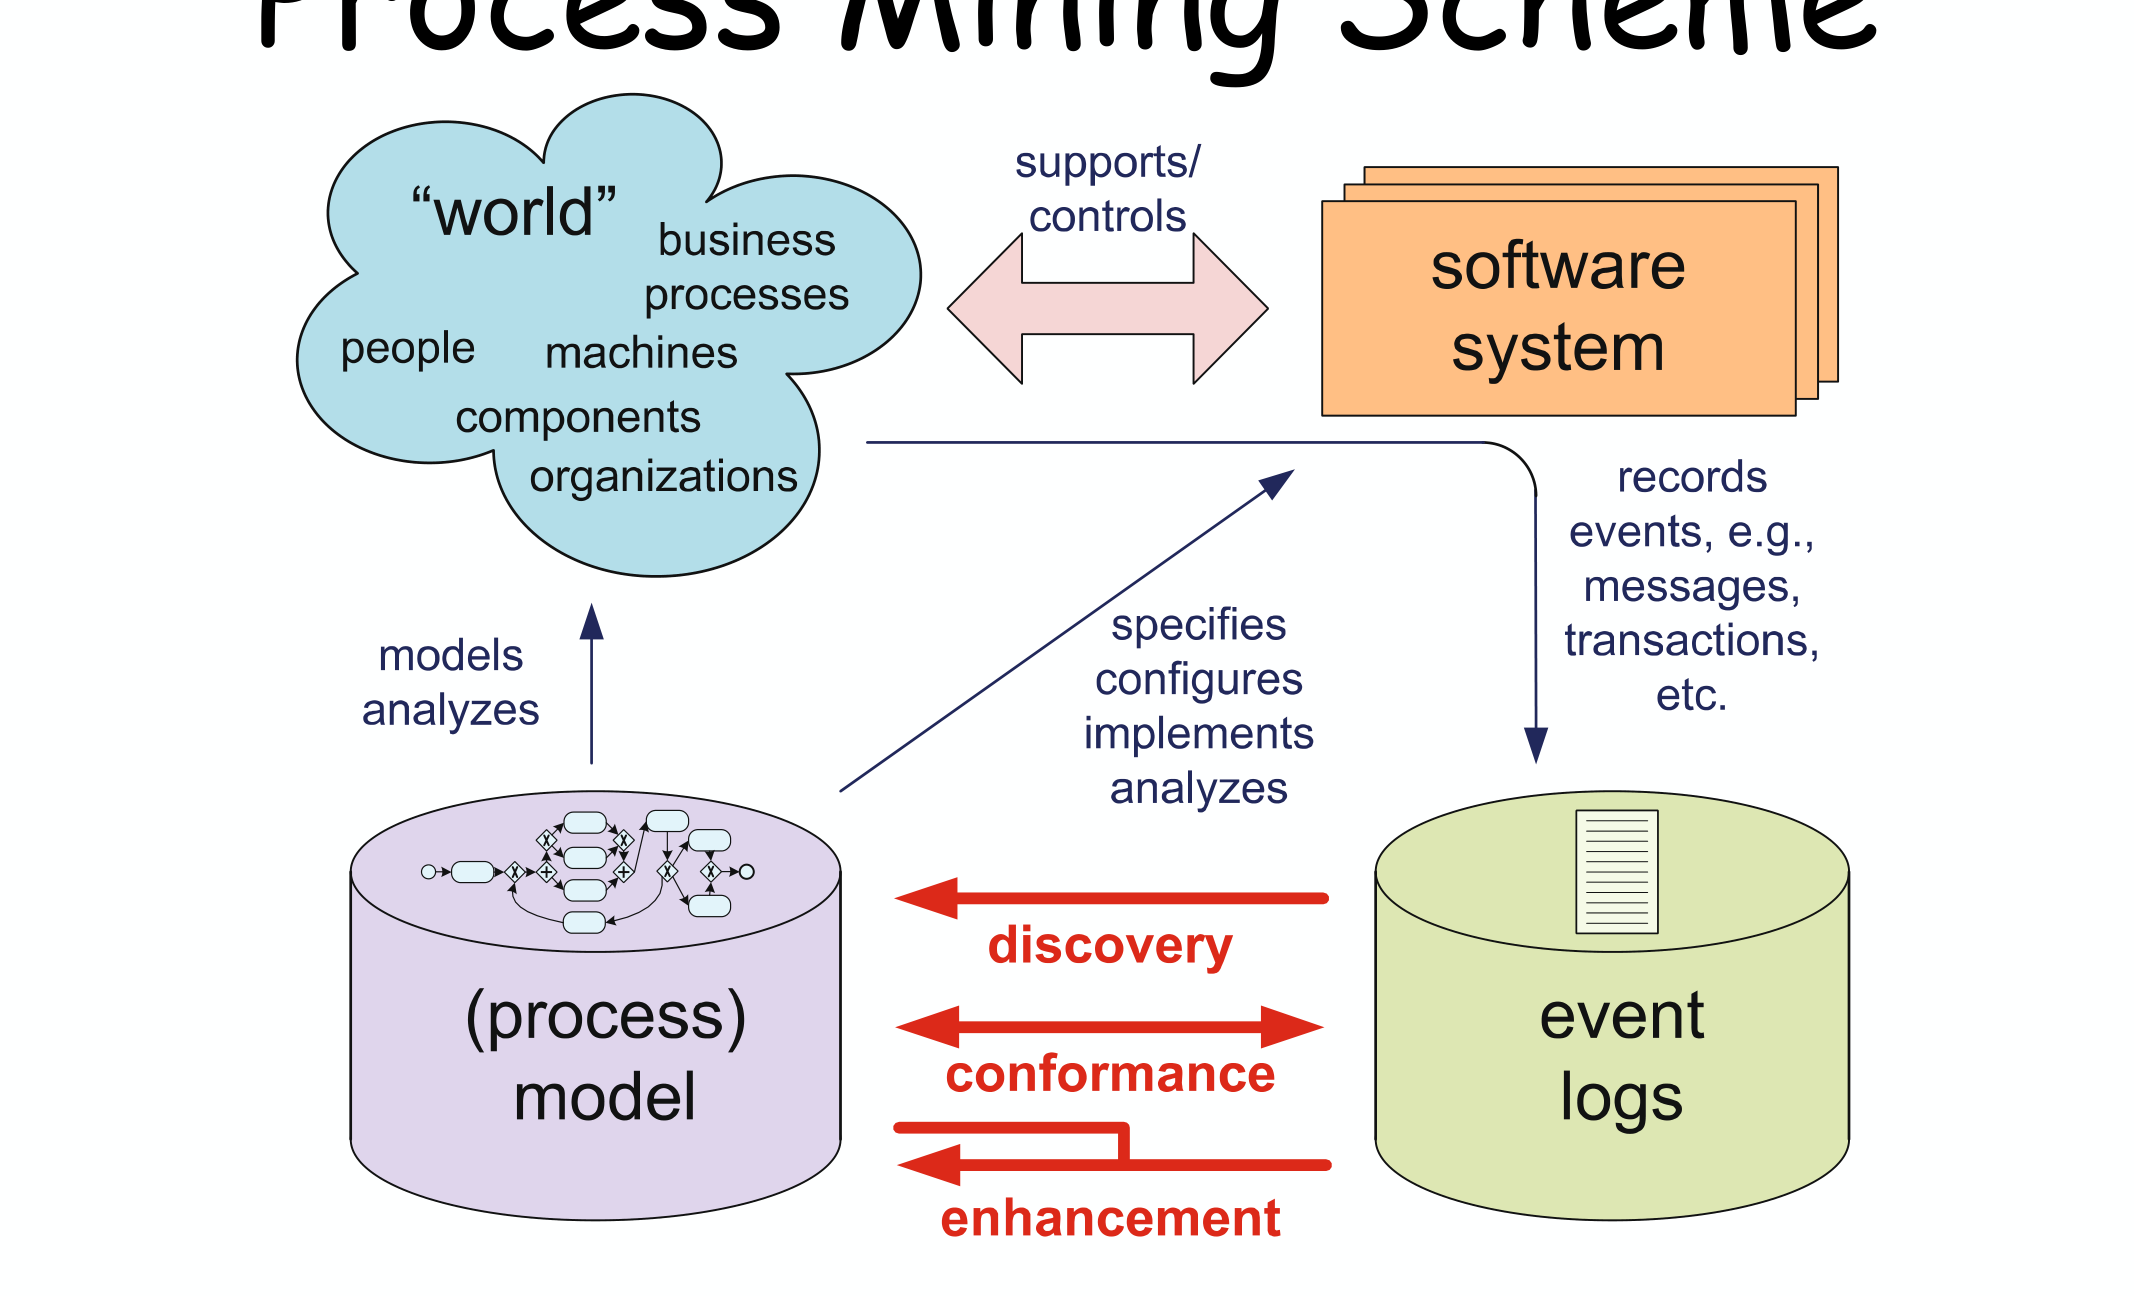
\includegraphics[width=0.74\linewidth,height=0.34\textheight,keepaspectratio]{images/05-mining_p14_scheme.png}
\caption{Lo schema. Il software system \textbf{supporta/controlla} il world e ne \textbf{registra gli eventi} negli event log. Il process model, da un lato, \textbf{modella e analizza} il world e, dall'altro, \textbf{specifica/configura} il software. Le tre frecce che collegano model ed event log sono le tre attività fondamentali del process mining: \textbf{discovery}, \textbf{conformance} ed \textbf{enhancement}.}
\end{figure}

Il concetto centrale è che il modello e i dati (l'event log) possono essere messi in relazione in tre modi diversi, e questi tre modi sono esattamente i tre tipi di process mining.

\begin{boxdefinition}{I tre tipi di process mining}
\begin{itemize}
\item \textbf{Discovery}: si parte da un event log e si produce un modello, \textbf{senza usare alcuna informazione a priori}. È il caso in cui non esiste ancora un modello e lo si vuole ricostruire dai dati. (Si chiama anche \emph{play-in}: dai dati al modello.)
\item \textbf{Conformance}: si confronta un modello \textbf{esistente} con un event log per misurare \textbf{quanto la realtà, registrata nel log, sia conforme al modello} (e viceversa). Serve a rilevare, localizzare e spiegare le deviazioni, e a misurarne la gravità.
\item \textbf{Enhancement}: si \textbf{estende o migliora} un modello esistente usando le informazioni sul processo reale contenute nel log. Non si limita a misurare la distanza (come la conformance), ma agisce sul modello.
\end{itemize}
\end{boxdefinition}

Un quarto termine utile è \textbf{replay} (o \emph{play-out}): far "girare" un modello su una traccia per vedere se il modello riesce a riprodurla. Il replay è alla base sia della conformance (le tracce del log sono riproducibili dal modello?) sia di analisi più avanzate come l'individuazione dei colli di bottiglia, i modelli predittivi e il supporto operativo.

Sull'enhancement vale la pena aggiungere una sottigliezza, perché quando modello e realtà divergono ci sono \textbf{due punti di vista opposti} su chi "ha torto".

\begin{boxnote}{Enhancement: i due angoli di visuale}
\begin{itemize}
\item Se il modello è pensato come \textbf{descrittivo}, una divergenza significa che \emph{il modello è sbagliato}: non cattura il comportamento reale, e la domanda è "come lo miglioro?". Un caso tipico è il \textbf{model repair}: se due attività sono modellate in sequenza ma nella realtà avvengono in qualsiasi ordine, si corregge il modello per rifletterlo.
\item Se il modello è pensato come \textbf{normativo} (prescrive come le cose \emph{dovrebbero} andare), una divergenza significa che \emph{la realtà si sta discostando dal desiderato}, e la domanda diventa "come controllo l'esecuzione perché rispetti il modello?".
\end{itemize}
\end{boxnote}

\section{\texorpdfstring{Gli event log: la materia prima}{Gli event log: la materia prima}}

Tutto il process mining si regge sull'\textbf{event log}. Per capire cosa contiene, servono quattro concetti annidati.

\begin{boxdefinition}{Process, case, event, attribute}
\begin{itemize}
\item Ogni \textbf{process} definisce un insieme di \textbf{case} (i casi trattati).
\item Ogni \textbf{case} è una serie di \textbf{event} (gli eventi che compongono quel caso).
\item Ogni \textbf{event} è un'istanza unica di un task del processo e si riferisce a \textbf{esattamente un case}. Gli eventi sono ordinati nel tempo tramite il loro \textbf{timestamp}.
\item Gli eventi possono avere \textbf{attribute}: per esempio \texttt{case id}, \texttt{activity}, \texttt{timestamp}, \texttt{duration}, \texttt{cost}, \texttt{resource}.
\end{itemize}
\end{boxdefinition}

Concretamente, un event log è una tabella: ogni riga è un evento, con colonne per case id, activity, timestamp, resource, cost, ecc. Due colonne sono essenziali: il \textbf{case id}, che lega l'evento al suo caso (cioè all'istanza di processo), e l'\textbf{activity}, che dice quale passo del processo è stato eseguito. Raggruppando gli eventi per case id e ordinandoli per timestamp, ogni caso diventa una \textbf{sequenza di attività}, cioè una \textbf{trace}.

Per lavorarci comodamente si passa a una rappresentazione compatta: si abbreviano le attività con lettere (per esempio \texttt{a} = register request, \texttt{b} = examine thoroughly, \texttt{c} = examine casually, \texttt{d} = check ticket, \texttt{e} = decide, \texttt{f} = reinitiate request, \texttt{g} = pay compensation, \texttt{h} = reject request) e ogni caso diventa una trace come $\langle a,b,d,e,h \rangle$. Un \textbf{event log} è quindi, in forma astratta, un insieme di trace.

\begin{boxdefinition}{Simple event log}
Sia $A$ un insieme di attività. Una \textbf{simple trace} $\sigma$ su $A$ è una sequenza finita di attività. Un \textbf{simple event log} $L$ su $A$ è un \textbf{multiset} di trace (multiinsieme, perché la stessa trace può ripetersi, e la sua \emph{molteplicità} conta). Notazione:

\[
L_1 = [\langle a,b,c,d\rangle^3,\ \langle a,c,b,d\rangle^2,\ \langle a,e,d\rangle]
\]

Significa tre casi con la prima trace, due con la seconda, uno con la terza.
\end{boxdefinition}

\section{\texorpdfstring{Discovery: dai dati al modello}{Discovery: dai dati al modello}}

La \textbf{discovery} prende un event log e ne ricava un modello di processo, senza informazioni a priori. L'idea intuitiva è leggere le trace e dedurne la struttura, riconoscendo pattern ricorrenti. Sul nostro esempio si ragiona così: tutti i casi iniziano con \texttt{a} e finiscono con \texttt{g} o \texttt{h}; ogni \texttt{e} è preceduto da \texttt{d} e da una delle due attività di esame (\texttt{b} o \texttt{c}); \texttt{e} è sempre seguito da \texttt{f}, \texttt{g} o \texttt{h}; \texttt{b}/\texttt{c} e \texttt{d} compaiono in ordini diversi, il che suggerisce che siano \textbf{in parallelo}; la ripetizione di \texttt{b/c, d, e} suggerisce un \textbf{loop} (attraverso \texttt{f}). Mettendo insieme queste osservazioni si costruisce una rete di Petri.

\begin{figure}[!htb]
\centering
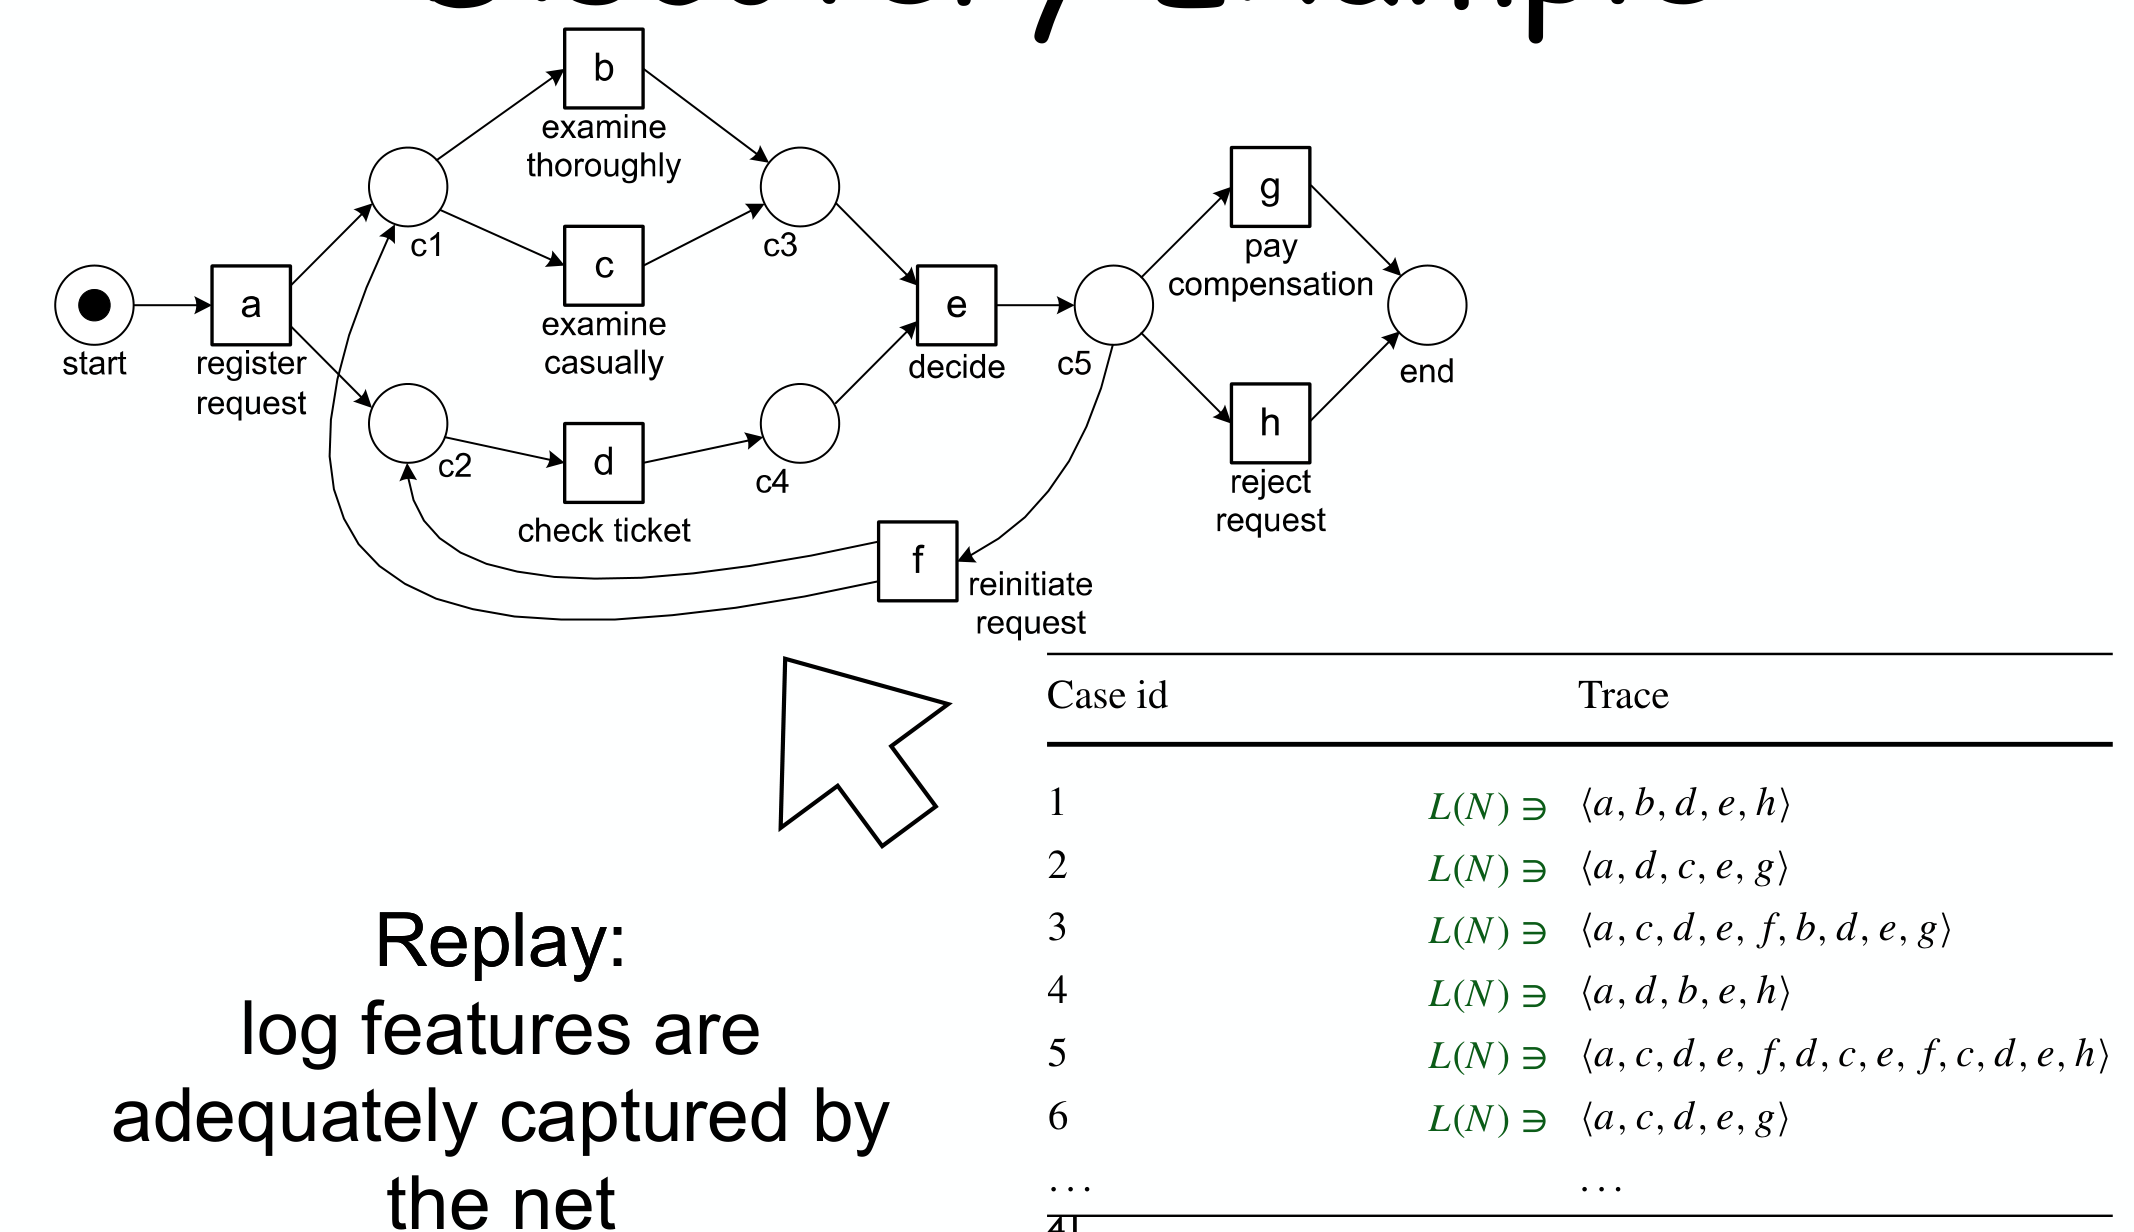
\includegraphics[width=0.74\linewidth,height=0.34\textheight,keepaspectratio]{images/05-mining_p40_discovery-example.png}
\caption{Discovery example. La rete ricostruita riproduce (replay) tutte le trace del log: la notazione $L(N) \ni \langle a,b,d,e,h\rangle$ indica che quella trace appartiene al linguaggio della rete, cioè è una sua esecuzione valida.}
\end{figure}

Un punto importante, che sembra un difetto ma è invece un \textbf{pregio}, è che la rete scoperta ammette anche trace \textbf{non presenti nel log} (per esempio $\langle a,d,c,e,f,b,d,e,g\rangle$). Questo è desiderato: l'obiettivo della discovery non è rappresentare \emph{esattamente} le trace campione osservate, ma \textbf{generalizzare} il comportamento del log per mostrare il modello sottostante più plausibile, quello che non verrà smentito dalle prossime osservazioni.

Nota: usiamo i Petri net per rappresentare i modelli scoperti perché sono un modo succinto di rappresentare i processi e hanno una semantica non ambigua ma intuitiva; ma alcune tecniche di mining si applicano anche ad altre rappresentazioni.

\section{\texorpdfstring{Qualità di un modello scoperto}{Qualità di un modello scoperto}}

Generalizzare troppo, o troppo poco, sono entrambi errori. È il problema centrale della discovery: trovare il giusto equilibrio.

\begin{boxwarning}{Overfitting e underfitting}
\begin{itemize}
\item \textbf{Overfitting}: il modello è \textbf{troppo specifico}, ammette solo il comportamento accidentale osservato nel log e nient'altro. Ha imparato "a memoria" i campioni.
\item \textbf{Underfitting}: il modello è \textbf{troppo generale}, ammette anche comportamenti del tutto scorrelati da quelli osservati.
\end{itemize}
\end{boxwarning}

L'esempio estremo di underfitting è la \textbf{flower net}: una rete in cui, dopo l'attività iniziale, tutte le attività pescano da un unico place centrale e possono avvenire in qualsiasi ordine e quante volte si vuole.

\begin{figure}[!htb]
\centering
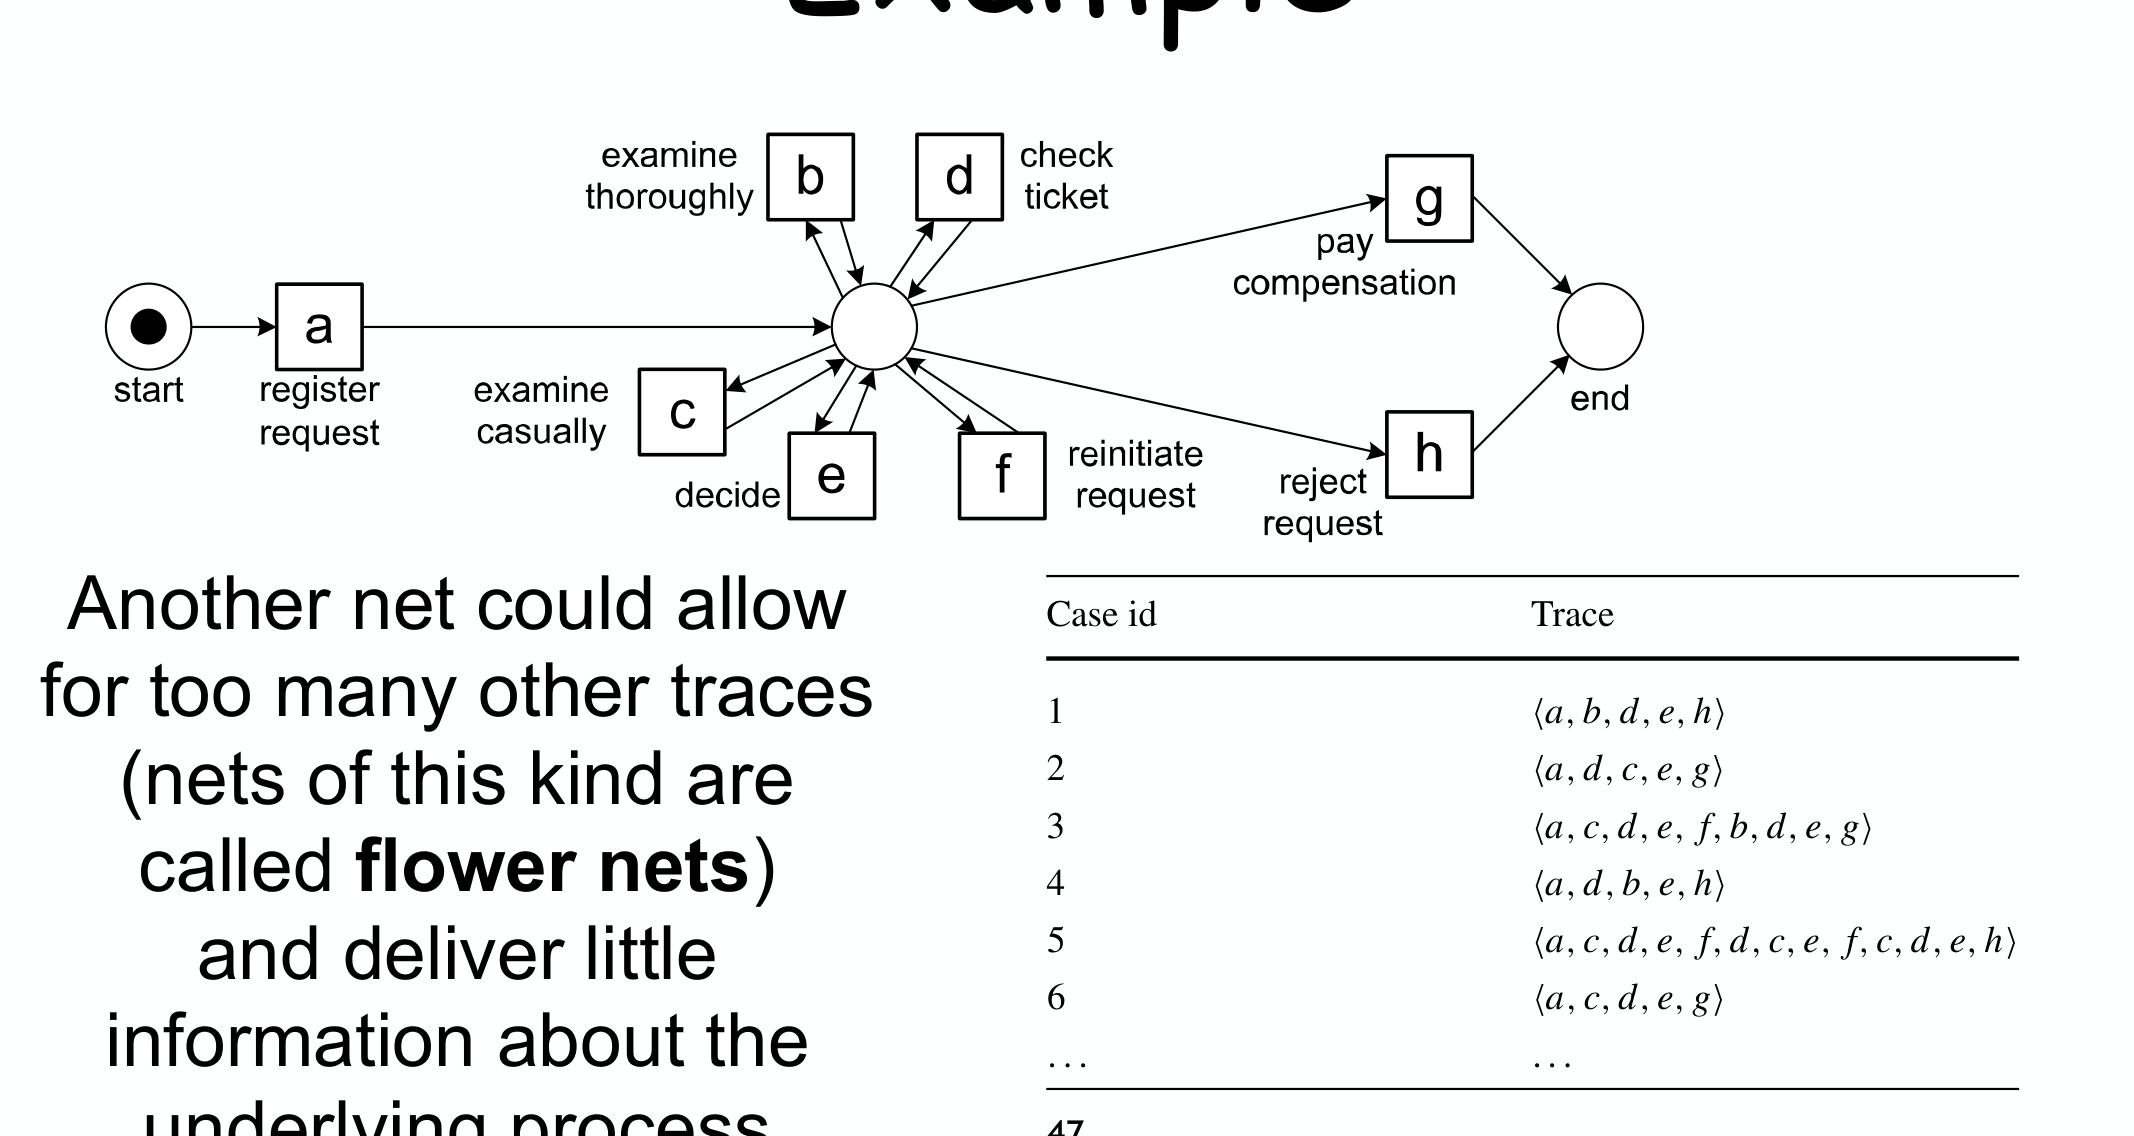
\includegraphics[width=0.74\linewidth,height=0.34\textheight,keepaspectratio]{images/05-mining_p46_flower-net.png}
\caption{Una \textbf{flower net}: ammette praticamente qualunque sequenza di attività. Riproduce tutte le trace del log (fitness perfetta) ma non dice \textbf{nulla} sulla struttura del processo — è l'underfitting portato all'estremo.}
\end{figure}

Per giudicare un modello si usano quindi \textbf{quattro criteri di qualità}, che vanno bilanciati tra loro:

\begin{itemize}
\item \textbf{Fitness} — il modello riesce a riprodurre (replay) le trace del log? Un modello con alta fitness spiega il comportamento osservato.
\item \textbf{Precision} — il modello evita di ammettere comportamenti \emph{troppo} diversi da quelli osservati? È l'opposto dell'underfitting.
\item \textbf{Generalization} — il modello generalizza oltre gli esempi specifici, senza incollarsi ai campioni? È l'opposto dell'overfitting.
\item \textbf{Simplicity} — il modello ha una struttura semplice? (Il principio del rasoio di Occam: a parità di potere esplicativo, meglio il modello più semplice.)
\end{itemize}

La \textbf{conformance} (che misura l'allineamento tra modello e realtà) si aggancia proprio alla fitness: su un esempio si può contare quante trace del log il modello riesce a riprodurre (per esempio "7 ok su 10" per un modello, "2 ok su 10" per un altro peggiore).

\section{\texorpdfstring{L'α-algorithm: scoprire una rete in modo automatico}{L'α-algorithm: scoprire una rete in modo automatico}}

Fin qui la discovery l'abbiamo fatta "a occhio". L'\textbf{α-algorithm} (alpha) è stato uno dei primi algoritmi di discovery capaci di gestire correttamente la \textbf{concorrenza}. Ha diversi limiti (li vedremo alla fine), ma è un'ottima introduzione, e molte sue idee sono confluite in tecniche più robuste. La sua strategia è di tipo \emph{play-in}: scandisce il log alla ricerca di particolari pattern, le \textbf{log-based ordering relations}, e con esse costruisce una rete.

\begin{boxdefinition}{Process discovery (formale)}
Un algoritmo di process discovery è una funzione che mappa un event log $L$ su un modello $M$ tale che $M$ sia \textbf{"rappresentativo"} del comportamento visto in $L$. Ci concentriamo su simple event log e su modelli Petri net (idealmente \textbf{sound workflow net}).
\end{boxdefinition}

\subsection{\texorpdfstring{Le relazioni d'ordine basate sul log}{Le relazioni d'ordine basate sul log}}

Tutto parte da una relazione elementare, il "segue direttamente".

\begin{boxdefinition}{Log-based ordering relations}
La relazione di base è il \textbf{directly-follows}:

\[
a >_L b
\]

Vale se esiste una trace $\sigma = \langle t_1,\dots,t_n\rangle$ in $L$ e un indice $i$ tale che $t_i = a$ e $t_{i+1} = b$ — cioè $a$ è (qualche volta) \textbf{immediatamente seguito} da $b$. Da questa si derivano tre relazioni:

\(\begin{aligned} a \to_L b &\quad \text{(causality): se } a >_L b \text{ ma non } b >_L a \\ a \#_L b &\quad \text{(mutual exclusion): se né } a >_L b \text{ né } b >_L a \\ a \parallel_L b &\quad \text{(concurrency): se } a >_L b \text{ e anche } b >_L a \end{aligned}\)

\begin{itemize}
\item \textbf{Causality} $a \to_L b$: l'ordine è sempre lo stesso $\rightarrow$ dipendenza causale (prima $a$, poi $b$).
\item \textbf{Mutual exclusion / no relation} $a \#_L b$: le due attività non sono mai adiacenti.
\item \textbf{Concurrency} $a \parallel_L b$: entrambi gli ordini compaiono $\rightarrow$ le due attività sono in parallelo (indipendenti).
\end{itemize}
\end{boxdefinition}

L'intuizione è che l'ordine (o il disordine) con cui due attività si susseguono nel log rivela la loro relazione strutturale nel processo:

\begin{figure}[!htb]
\centering
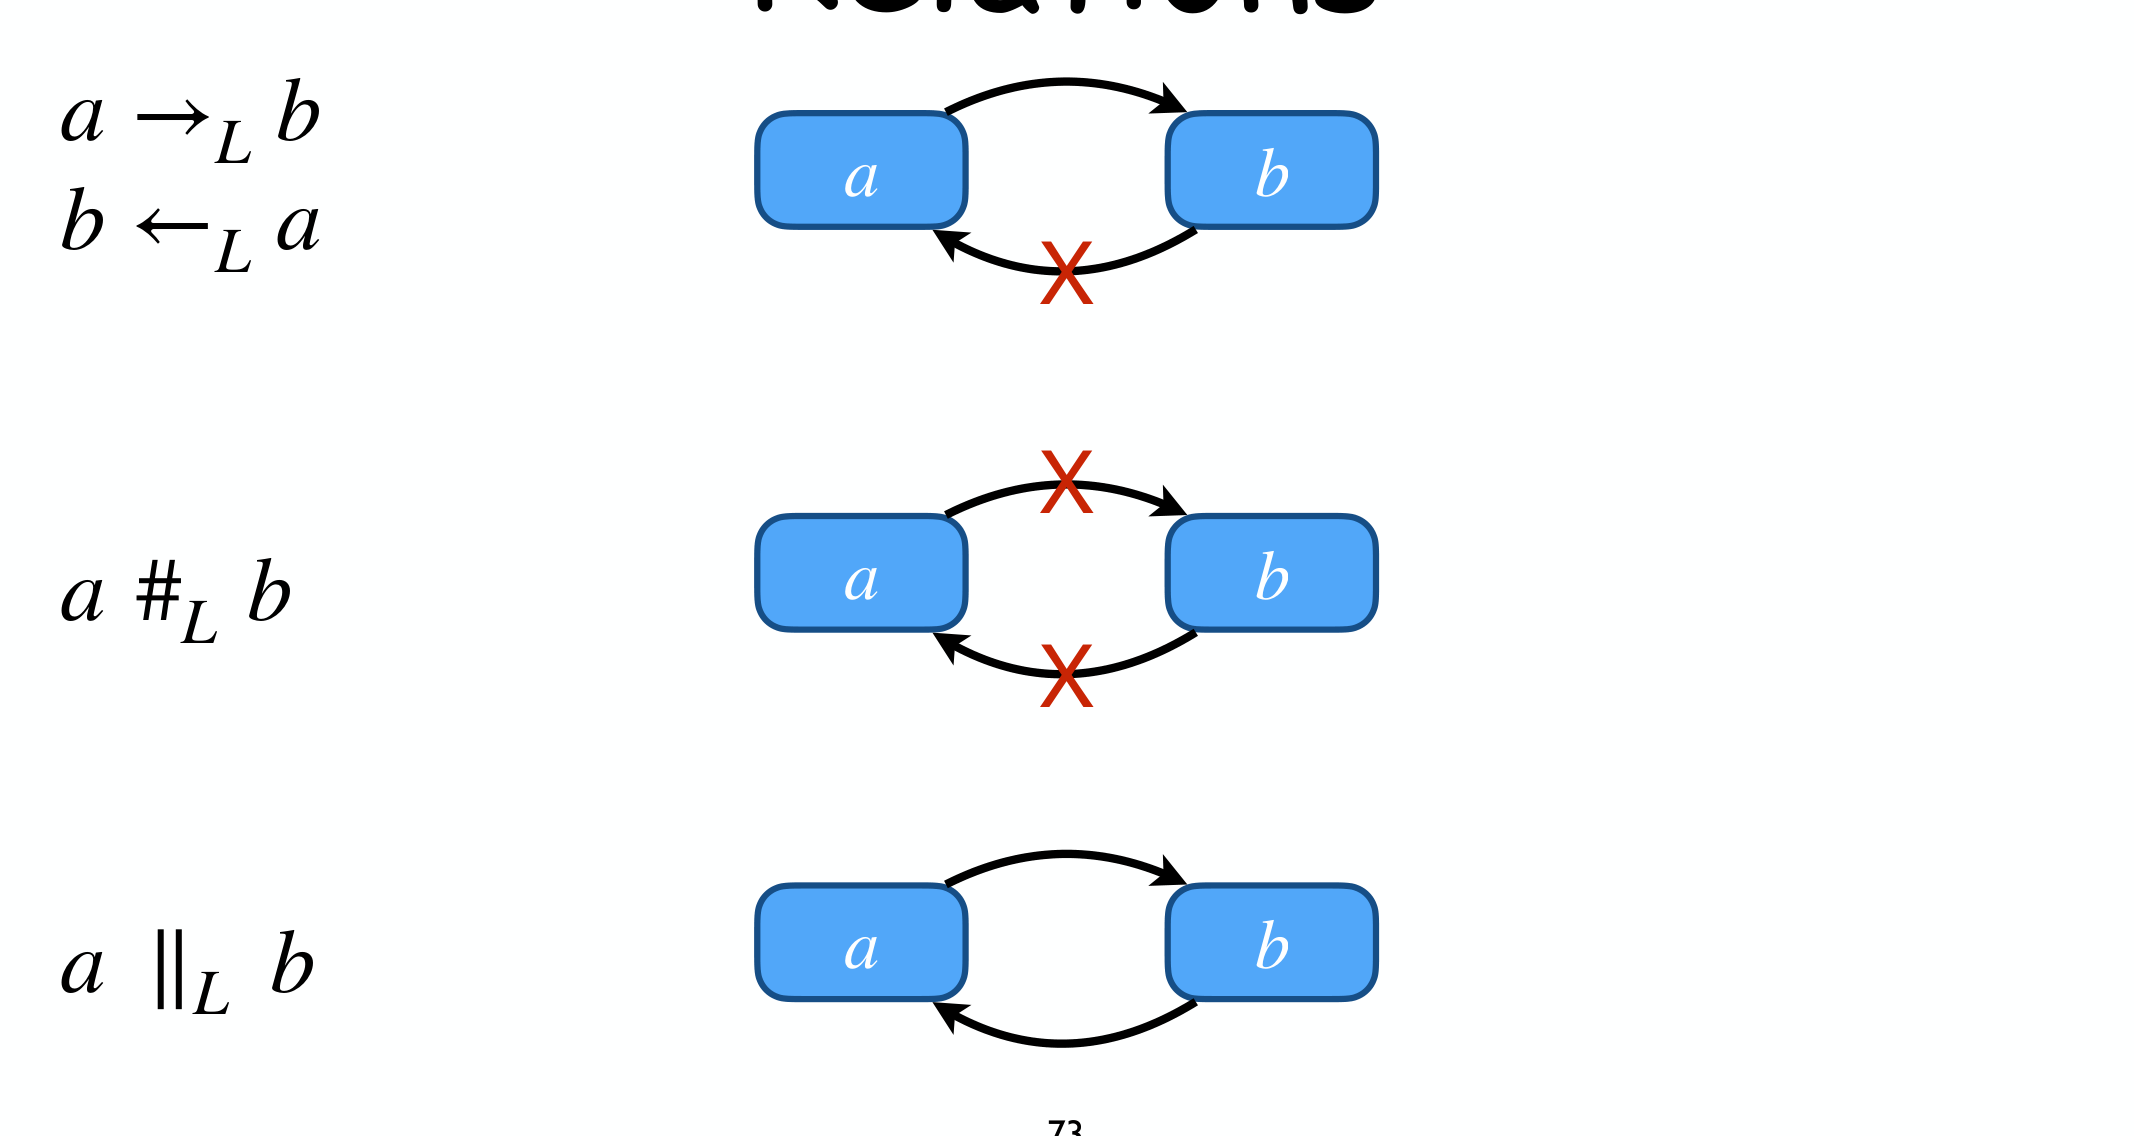
\includegraphics[width=0.74\linewidth,height=0.34\textheight,keepaspectratio]{images/05-mining_p72_ordering-relations.png}
\caption{Le relazioni. $a \to_L b$: si osserva solo $a$ seguito da $b$ (causalità). $a \#_L b$: mai adiacenti. $a \parallel_L b$: si osservano entrambi gli ordini, segno di parallelismo.}
\end{figure}

Se disegniamo un nodo per attività e un arco $a \to b$ ogni volta che $a >_L b$, otteniamo un \textbf{Directly-Follows Graph (DFG)}, una prima rappresentazione grezza del comportamento (opzionalmente con archi pesati dalle frequenze).

\subsection{\texorpdfstring{La footprint matrix}{La footprint matrix}}

Tutte le relazioni d'ordine di un log si raccolgono in modo compatto in una \textbf{footprint matrix}: una tabella con una riga e una colonna per ogni attività, dove ogni cella riporta la relazione tra le due attività corrispondenti.

\begin{figure}[!htb]
\centering
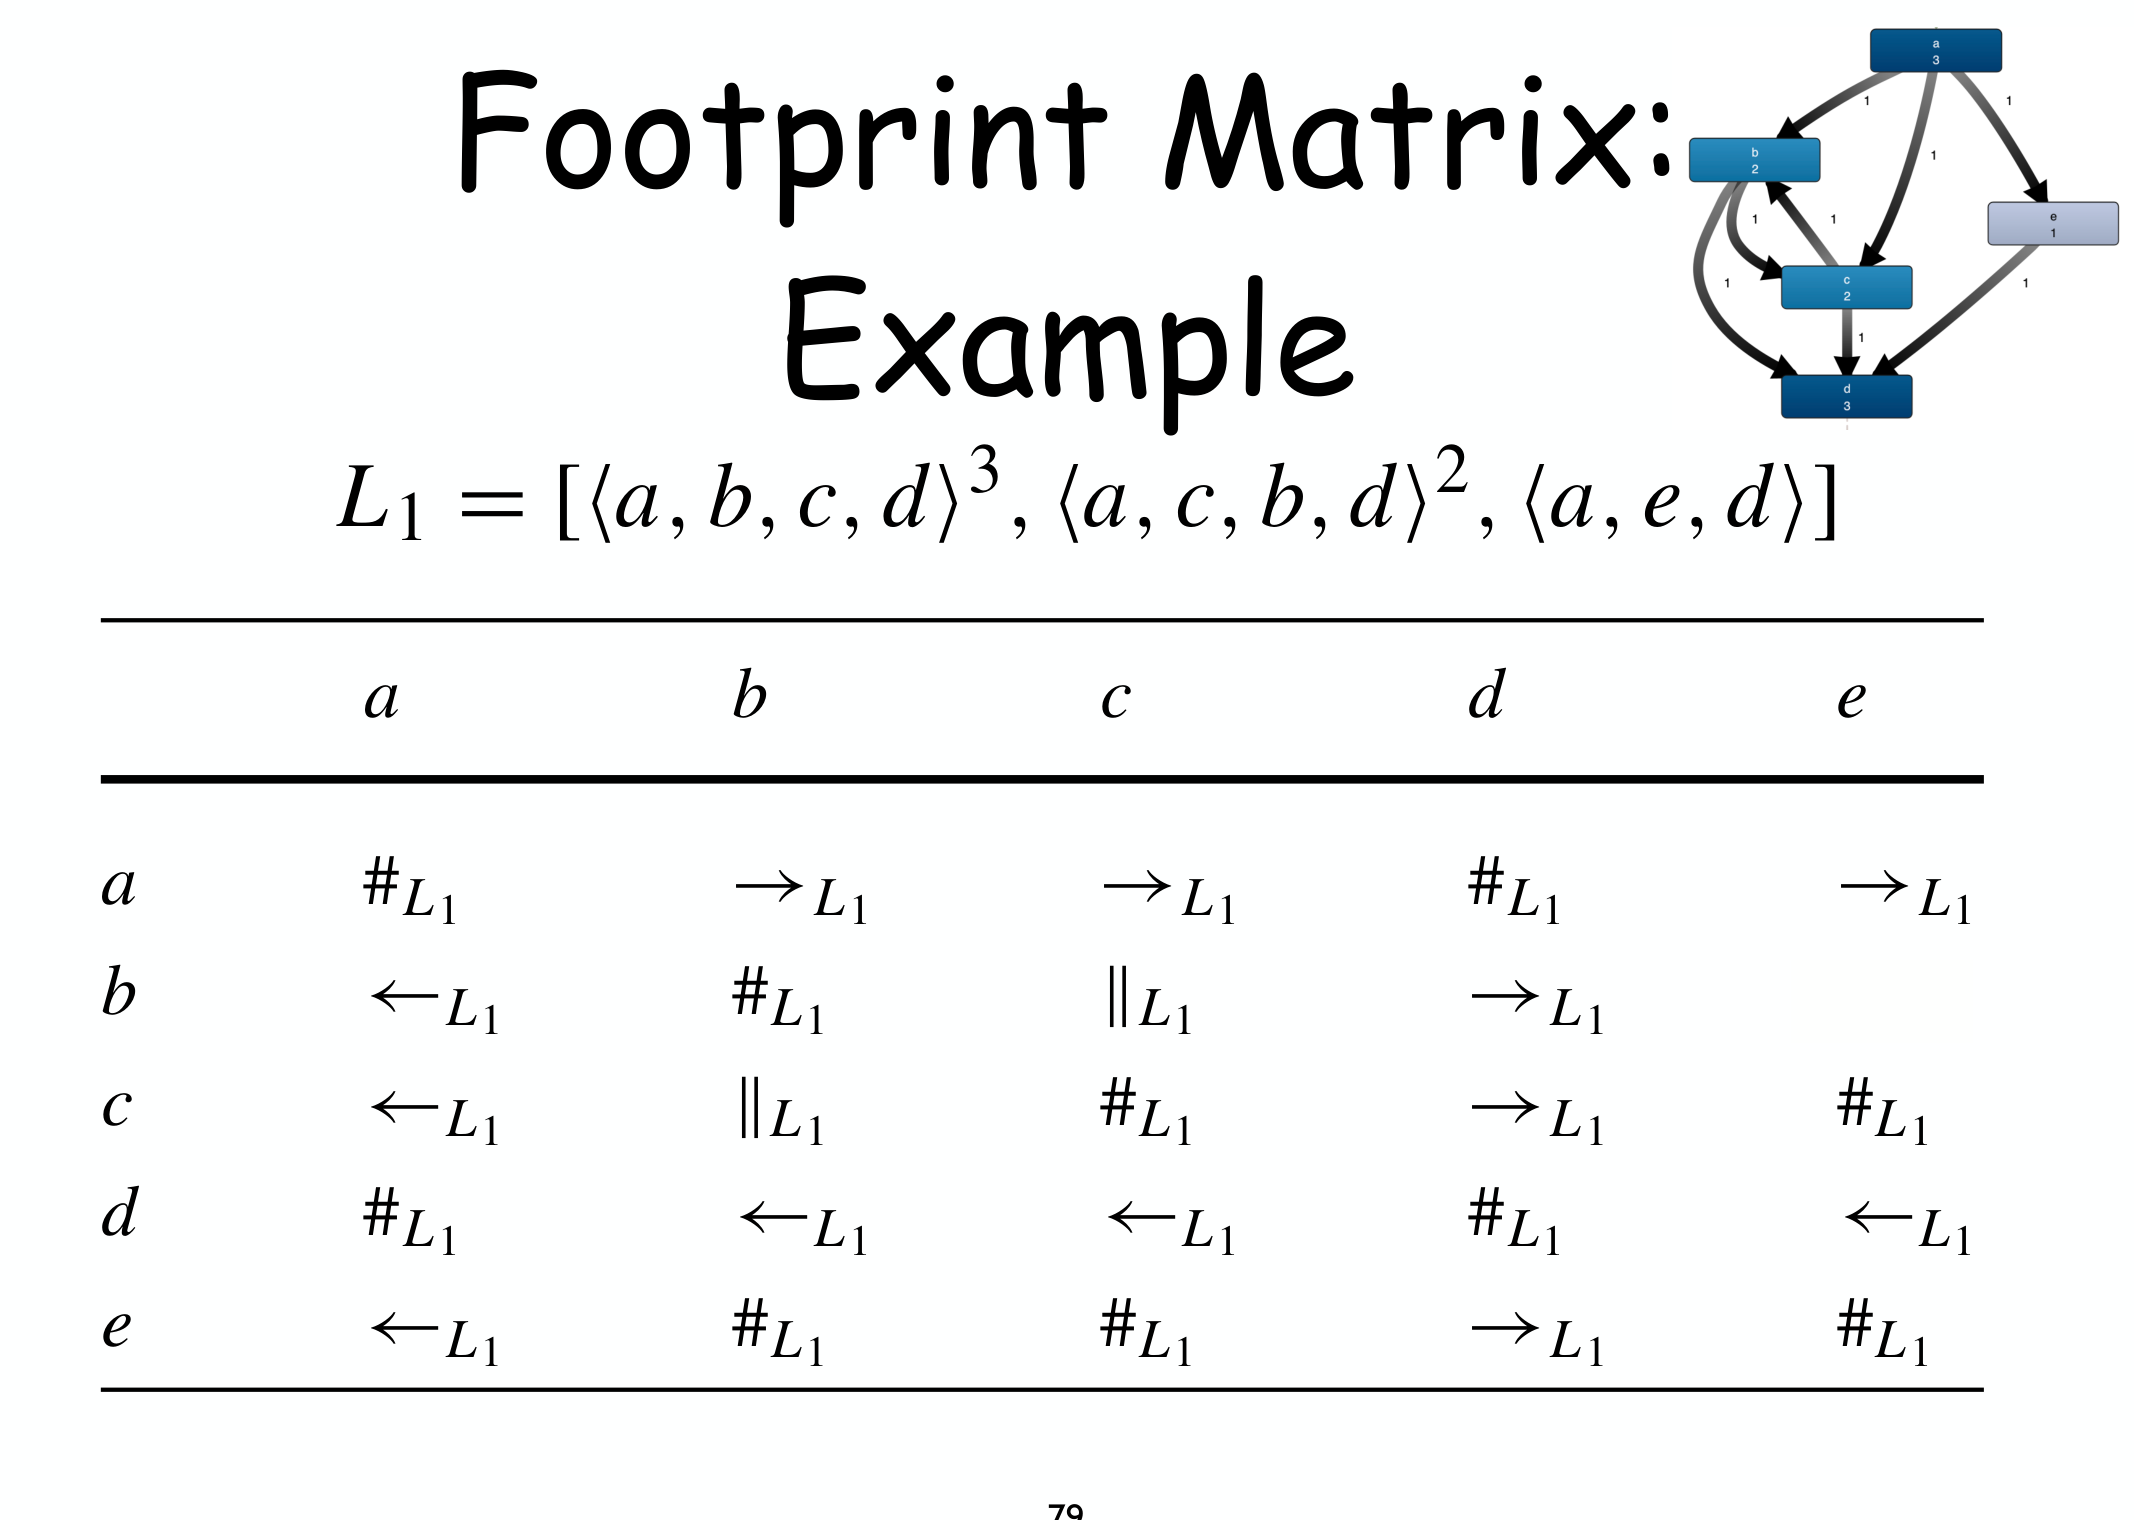
\includegraphics[width=0.74\linewidth,height=0.34\textheight,keepaspectratio]{images/05-mining_p78_footprint-matrix.png}
\caption{La footprint matrix del log $L_1$. È \textbf{antisimmetrica} rispetto alla diagonale per le relazioni causali (se in $(a,b)$ c'è $\to$, in $(b,a)$ c'è $\leftarrow$), mentre $\#$ e $\parallel$ sono simmetriche. La cella $(b,c) = \parallel$ dice che $b$ e $c$ sono concorrenti.}
\end{figure}

\subsection{\texorpdfstring{I passi dell'algoritmo}{I passi dell'algoritmo}}

L'α-algorithm costruisce la rete $\alpha(L) = (P_L, T_L, F_L)$ in otto passi. L'idea di fondo è che ogni \textbf{place} della rete corrisponde a un "punto di decisione" tra un gruppo di attività che lo alimentano e un gruppo che ne consuma.

\begin{boxdefinition}{I passi dell'α-algorithm}
\begin{enumerate}
\item \textbf{$T_L$} — una transizione per ogni attività che compare nel log.
\item \textbf{$T_I$} — le attività che compaiono come \textbf{prima} (first) di almeno una trace: gli eventi iniziali.
\item \textbf{$T_O$} — le attività che compaiono come \textbf{ultima} (last) di almeno una trace: gli eventi finali.
\item \textbf{$X_L$} — le coppie di insiemi $(A, B)$ tali che \textbf{ogni} $a \in A$ è in causalità con \textbf{ogni} $b \in B$ ($a \to_L b$), tutte le attività di $A$ sono mutuamente esclusive tra loro ($\#_L$), e così tutte quelle di $B$. Sono i candidati "punti di decisione" (place).
\item \textbf{$Y_L$} — si tengono solo le coppie \textbf{massimali} di $X_L$ (quelle non contenute in un'altra): $(A,B)$ con $A$ e $B$ i più grandi possibile.
\item \textbf{$P_L$} — un place $p_{(A,B)}$ per ogni coppia in $Y_L$, più il place iniziale $i_L$ e quello finale $o_L$.
\item \textbf{$F_L$} — gli archi: da ogni $a \in A$ al place $p_{(A,B)}$, dal place a ogni $b \in B$; inoltre da $i_L$ verso ogni transizione iniziale ($T_I$) e da ogni transizione finale ($T_O$) verso $o_L$.
\item \textbf{$\alpha(L) = (P_L, T_L, F_L, i_L)$} — la rete risultante.
\end{enumerate}
\end{boxdefinition}

I passi 4 e 5 sono il cuore dell'algoritmo. Il passo 4 cerca ogni possibile "gruppo di cause $A$ $\rightarrow$ gruppo di effetti $B$" compatibile con la footprint; il passo 5 tiene solo i gruppi più grandi, perché un place che collega insiemi più ampi cattura meglio la struttura (un place per $(\{a\},\{b,e\})$ è più informativo di uno per $(\{a\},\{b\})$ e uno per $(\{a\},\{e\})$ separati). Applicato al log $L_1$ dell'esempio, l'algoritmo produce questa rete:

\begin{figure}[!htb]
\centering
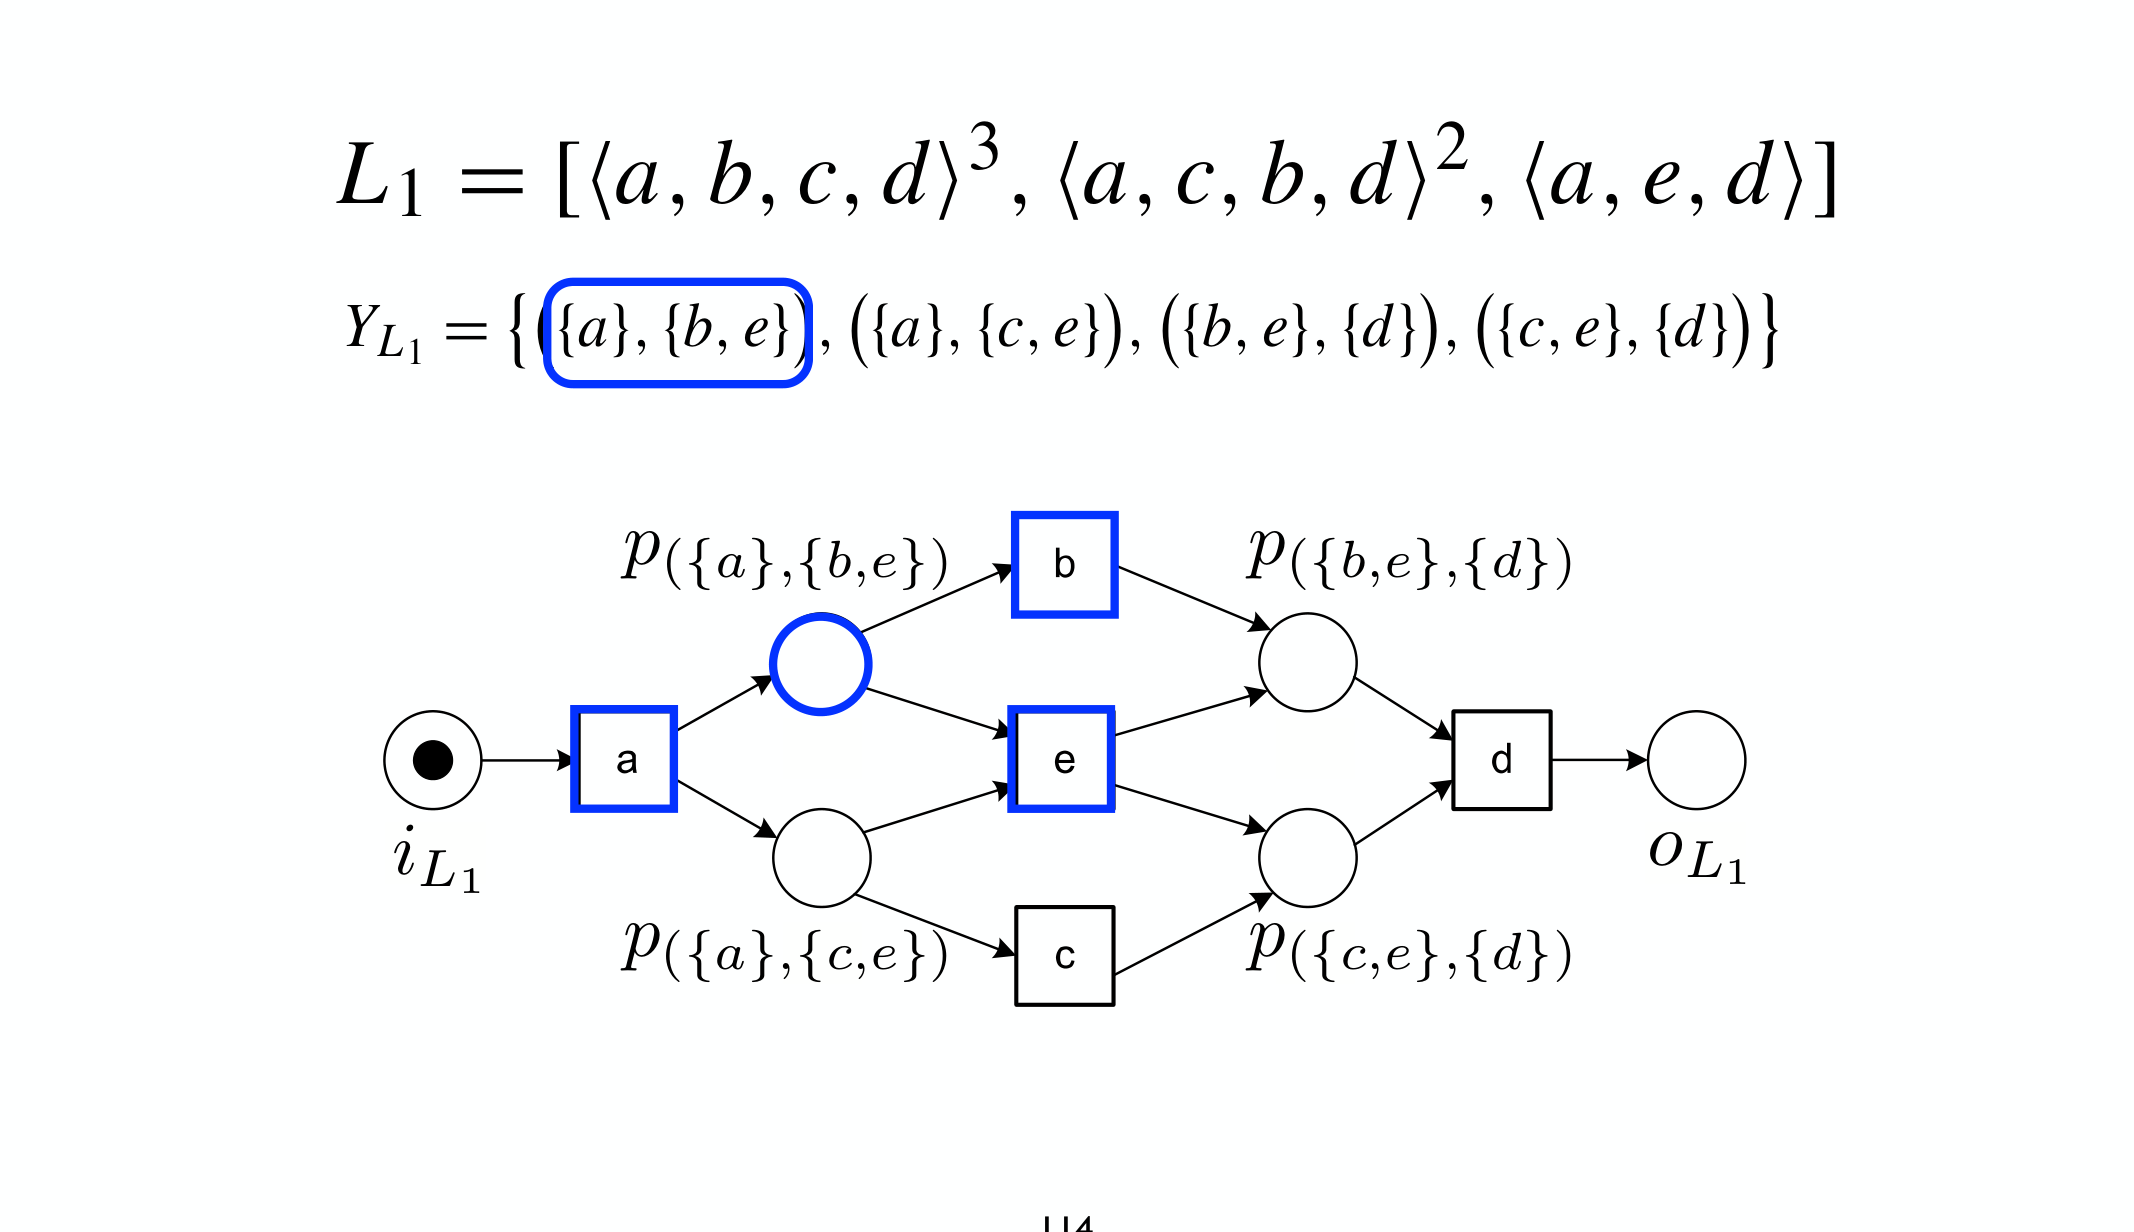
\includegraphics[width=0.74\linewidth,height=0.34\textheight,keepaspectratio]{images/05-mining_p113_alpha-net.png}
\caption{La rete $\alpha(L_1)$ costruita ai passi 6-7. I place massimali di $Y_{L_1} = \{(\{a\},\{b,e\}), (\{a\},\{c,e\}), (\{b,e\},\{d\}), (\{c,e\},\{d\})\}$ diventano i nodi cerchio della rete, collegati alle transizioni secondo il passo 7.}
\end{figure}

\section{\texorpdfstring{I limiti dell'α-algorithm}{I limiti dell'α-algorithm}}

L'algoritmo è elegante ma fragile. Conviene conoscerne i limiti, perché mostrano cosa un semplice conteggio di adiacenze \emph{non} riesce a catturare.

\begin{boxwarning}{Tre limiti principali}
\begin{itemize}
\item \textbf{Dipendenze implicite}: alcune dipendenze non-locali (place "ridondanti" che vincolano scelte lontane nel processo) non vengono ricostruite, perché la footprint guarda solo alle adiacenze dirette.
\item \textbf{Short loop}: i cicli corti (un'attività che si ripete immediatamente, come \texttt{b,b}, o cicli di lunghezza due) confondono l'algoritmo — un'attività può risultare "sconnessa" dal modello, perché $a \parallel_L a$ non è distinguibile da un vero parallelismo.
\item \textbf{Noise}: l'algoritmo \textbf{non tiene conto delle frequenze}. Un comportamento raro e infrequente (rumore, non necessariamente un errore) pesa quanto uno comune: non c'è modo, di per sé, di decidere se ignorare le trace meno frequenti.
\end{itemize}
\end{boxwarning}

Il process mining chiude il cerchio del corso: dopo aver imparato a \emph{disegnare} processi (\hyperref[ch:03]{03 — Visual Notation}) e a dar loro una \emph{semantica} (\hyperref[ch:04]{04 — Petri Nets}), ora sappiamo anche \emph{ricavarli dai dati} e \emph{misurarne la qualità}. Nelle prossime lezioni torneremo sull'analisi strutturale delle reti. $\rightarrow$ \hyperref[ch:06]{06 — Orchestration e Collaboration}